\documentclass[]{DINOReportMemo}
\usepackage{DINO_C-REx}
\usepackage{colortbl}


\newcommand{\ModuleName}{Image Generation} %edit this!
\newcommand{\subject}{Camera Object Unit Tests} %edit this!
\newcommand{\status}{Initial Version}
\newcommand{\preparer}{Matt Muszynski} %edit this!
\newcommand{\summary}{Description of unit tests completed for the DINO C-REx camera object. This includes tests 4.8 through 4.18.} %edit this
\usepackage{float}
\usepackage{rotating}
\usepackage{pdflscape}
\usepackage{wasysym}
\begin{document}

\makeCover


%
% enter the revision documentation here
% to add more lines, copy the table entry and the \hline, and paste after the current entry.
%
\pagestyle{empty}
{\renewcommand{\arraystretch}{2}
\noindent
\begin{longtable}{|p{0.5in}|p{4.5in}|p{1.14in}|}
\hline
{\bfseries Rev}: & {\bfseries Change Description} & {\bfseries By} \\
\hline
1.0 & Initial Release & Matt Muszynski \\ %edit this
\hline

\end{longtable}
}

\newpage
\setcounter{page}{1}
\pagestyle{fancy}

\tableofcontents
~\\ \hrule ~\\

\newpage
\section{Overview}\\\\
This document describes all unit tests written for the image object by the DINO C-REx camera model team. Each method of the image object has an associated test, and additional integrated tests are performed where deemed useful by the team. Each test has an entry in this document for status (including date of status change), responsible DINO C-REx team member, a qualitative description of the test performed and a brief technical discussion of the method employed in code to achieve the test. Because it is used in the image.update\_state() method, tests for em.planck() are also recorded in this document.

\section{Tests}
\subsection{Test 4.8: image.find\_stars\_in\_FOV()}
\textbf{Status}: Incomplete. 10.31.17\\
\textbf{Responsible Team Member}: Matt Muszynski \\
\textbf{Description}: This method is responsible for limiting objects to only those in the field of view of the camera. Here, an image calculated at run time is compared to known star catalogs to ensure all expected stars (above a reasonable magnitude) are present.\\
\textbf{Method}: \\

\subsection{Test 4.9: image.remove\_occulatations()}
\textbf{Status}: Incomplete. 10.31.17\\
\textbf{Responsible Team Member}: Matt Muszynski \\
\textbf{Description}: To test this method, an extended spherical body is placed in the center of a frame. We then check all stars that should be present in that frame and ensure that all objects closer to the center of the frame than half the object's angular size are appropriately removed.\\
\textbf{Method}: 
\begin{enumerate}
    \item Set up the test.
    \begin{enumerate}
        \item Set the position of a body (named Earth) to be $\vec{r}_{earth} = [1 au, 0, 0]$, the position of the spacecraft to be $\vec{r}_{s/c} = [1 au - 250000 km, 0, 0]$, and give the spacecraft an attitude DCM of $
        \begin{bmatrix}
        1 & 0 & 0 \\ 0 & 1 & 0 \\ 0 & 0 & 1
        \end{bmatrix}$. This puts the spacecraft 250,000 km from the Earth pointing so that the earth is at the exact center of its field of view. Because the camera to body DCM is also an identity matrix, the camera points exactly where the spacecraft does.
        \item Set the camera debug messages such that occulted stars are removed, but the resolved body is not added.
        \item Take an image with a single frame by setting taekImage to 1, running starCam.updateState(), setting takeImage to 0, and running starCam.updateState() one more time.
        \item Set the camera debug messages such that occulted stars are not removed, and the resolved body is not added.
        \item Take an image with a single frame by setting taekImage to 1, running starCam.updateState(), setting takeImage to 0, and running starCam.updateState() one more time. Now we have two images, one with all the stars in the FOV including those that are occulted, and one without those that are occulted.
    \end{enumerate}
    \item Test that no non-occulted stars are closer to the center of the FOV than the limb of the earth.
    \begin{enumerate}
        \item For every non-occulted star, find the distance between the center of the FOV and where it appears on the focal plane.
        \item Project phsical distance into angular distance
        \item Calculate angular distance between the center of the FOV and the limb of the earth.
        \item Assert that none of the non-occulted stars are closer to the center of the FOV than the limb of the earth.
    \end{enumerate}
    \item Test that no occulted stars are farther to the center of the FOV than the limb of the earth.
    \begin{enumerate}
        \item Compare the image above with all stars with the image with only non-occulted stars. Use this to create a set of only occulted stars.
        \item Assert that the lengths of the array containing occulted stars and the array containing non-occulted stars sum to the length of the array of all stars from image where occulted stars were not removed.
        \item Find physial distance between center of FOV and each occulted star.
        \item Project that physical distance into angular distance in the FOV.
        \item Assert that none of the non-occulted stars are farther from the center of the FOV than the limb of the earth.
    \end{enumerate}

\end{enumerate}
\begin{figure*}[t!]
    \centering
    \begin{subfigure}
        \centering
        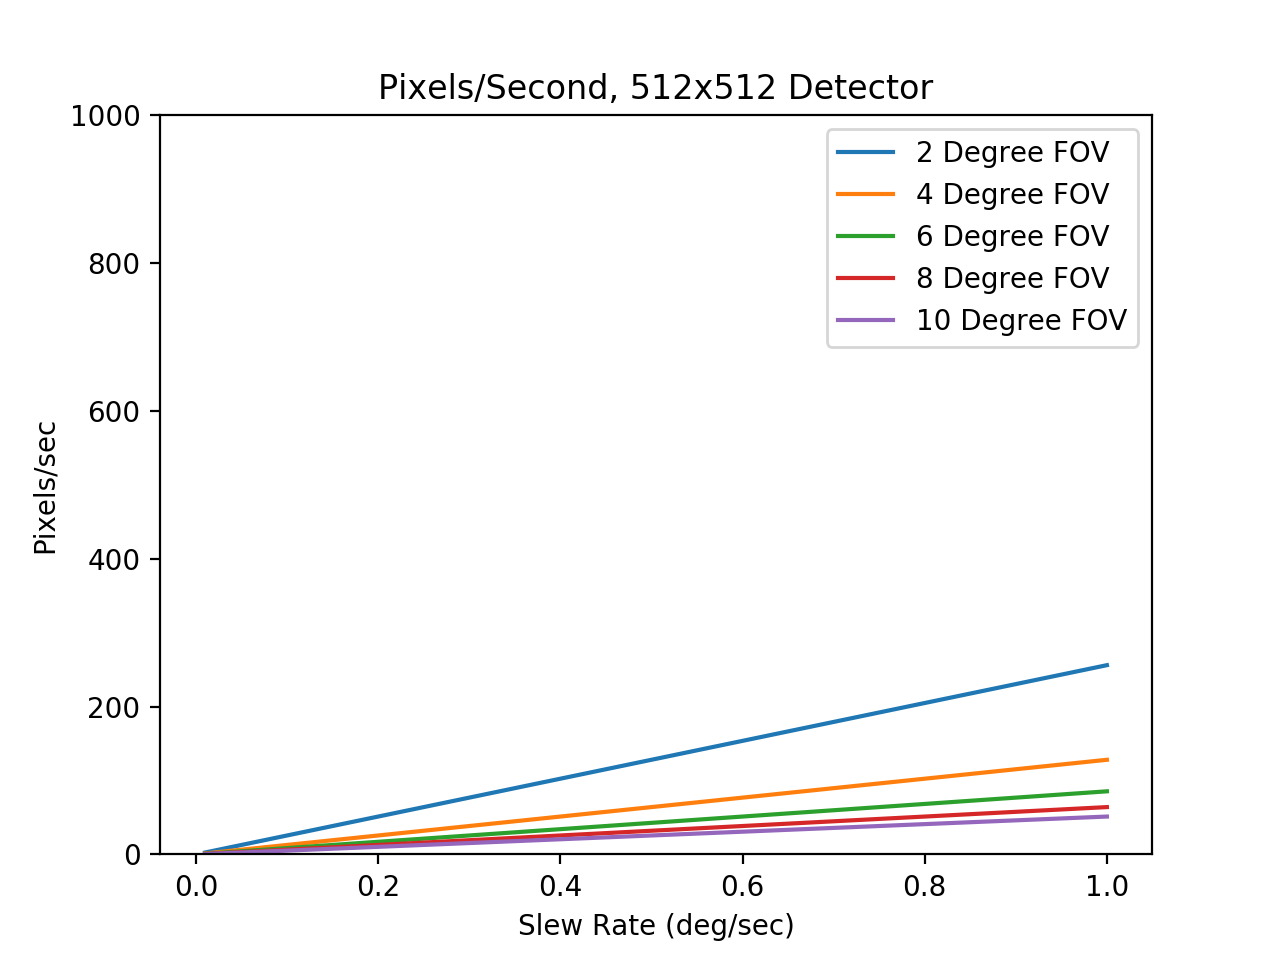
\includegraphics[height=2.1in]{512x512_pix_per_sec}
    \end{subfigure}%
    ~ 
    \begin{subfigure}
        \centering
        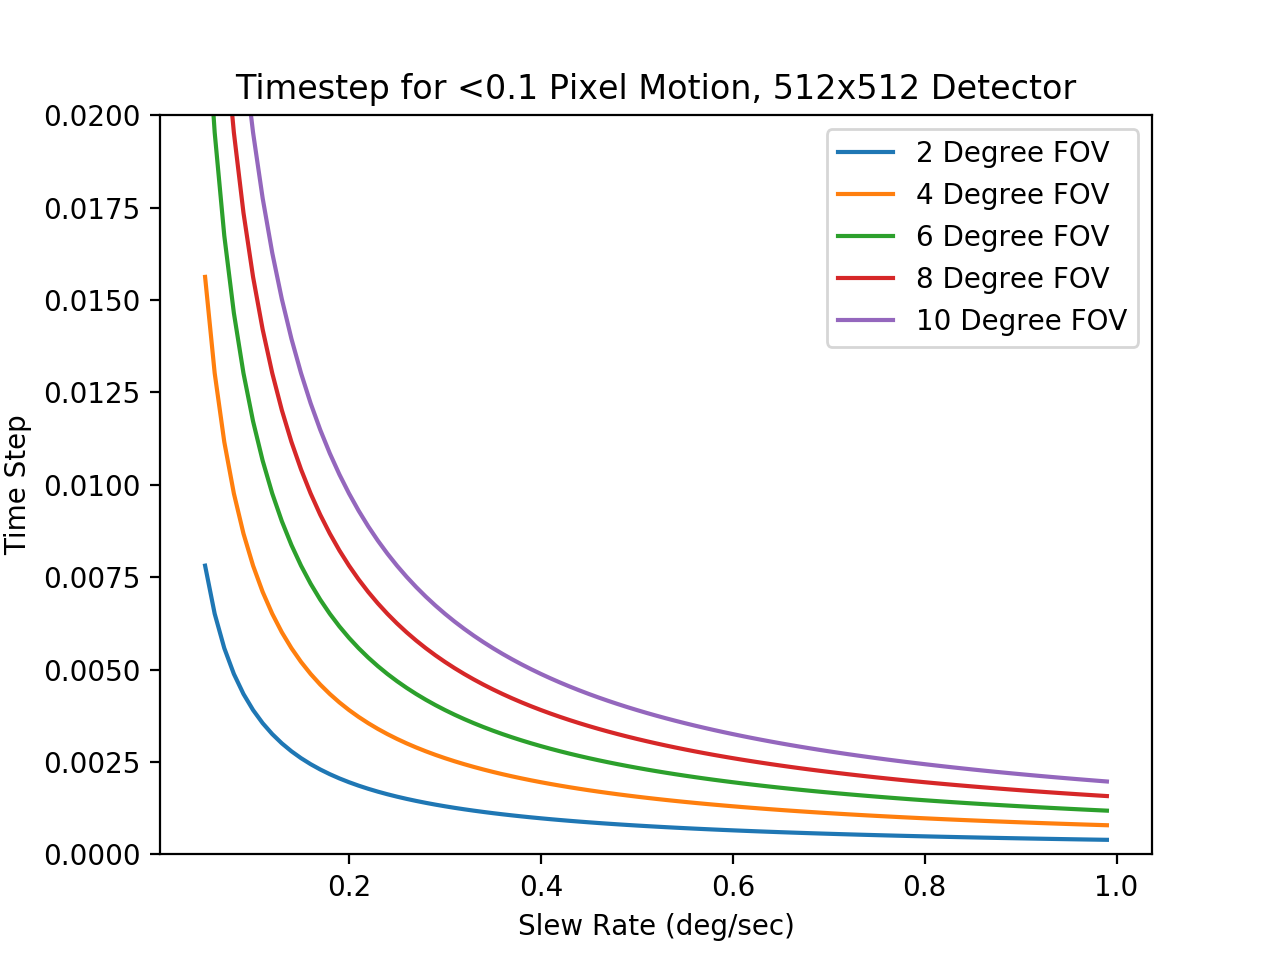
\includegraphics[height=2.1in]{512x512_min_dt}
    \end{subfigure}
    \caption{Best case plots show many solutions for $512\times512$ camera.}
    \label{512}
\end{figure*}

\begin{figure*}[t!]
    \centering
    \begin{subfigure}
        \centering
        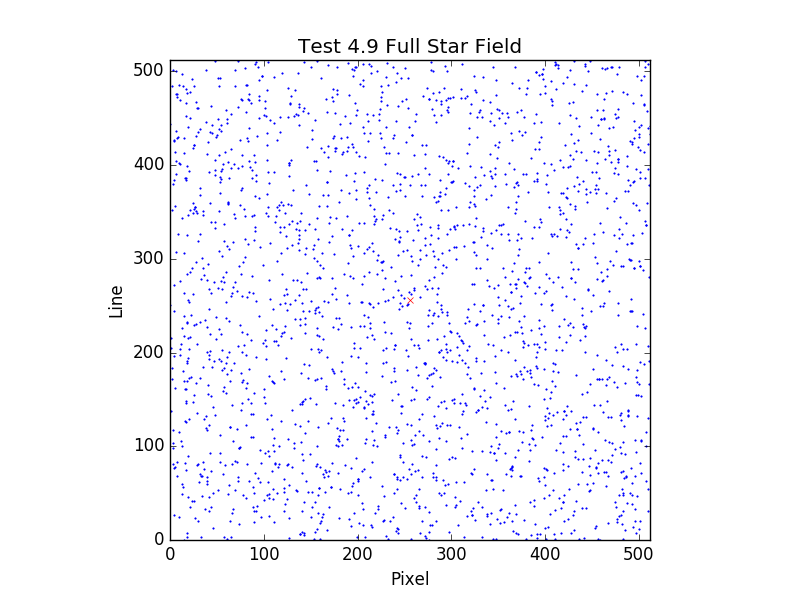
\includegraphics[height=1.5in]{fullNoHole}
    \end{subfigure}%
    ~ 
    \begin{subfigure}
        \centering
        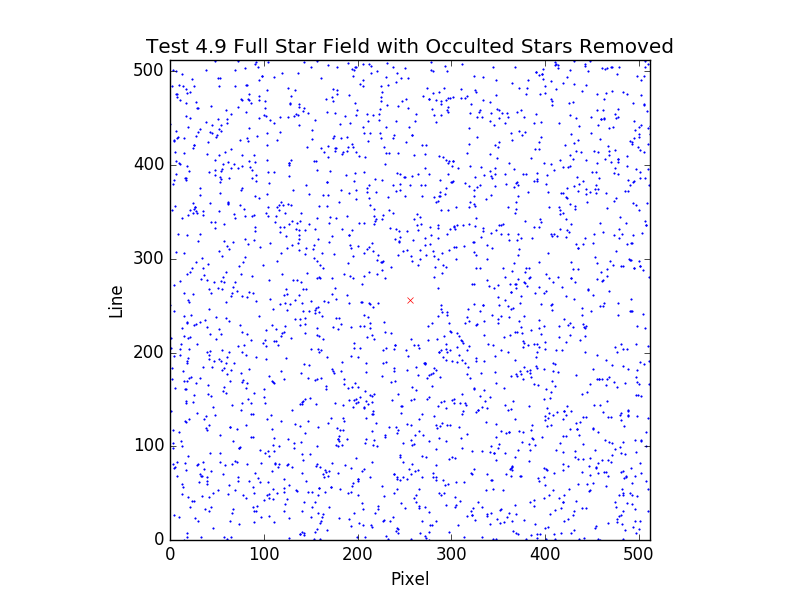
\includegraphics[height=1.5in]{fullWithHole}
    \end{subfigure}
    ~ 
    \begin{subfigure}
        \centering
        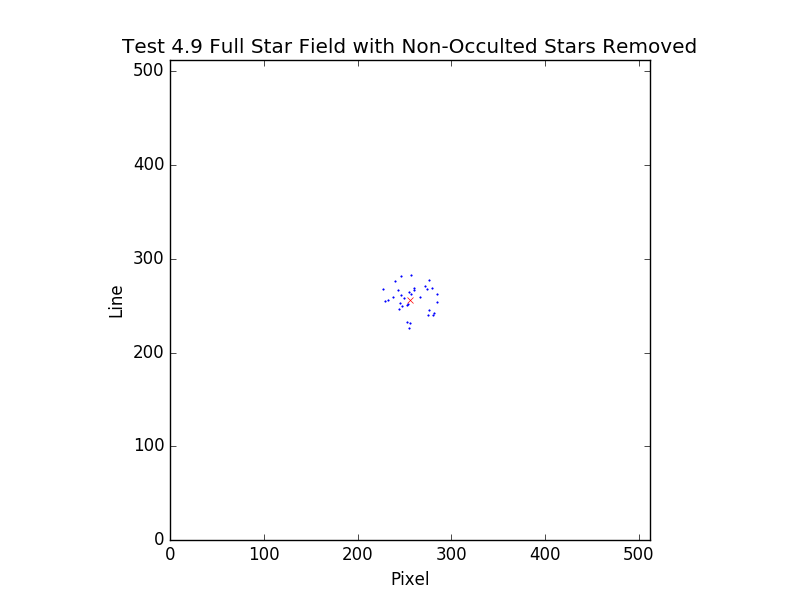
\includegraphics[height=1.5in]{fullWithFill}
    \end{subfigure}
    \caption{All stars used in test 4.9. Images show full star field, set of non-occulted stars, and set of occulted stars.}
    \label{512}
\end{figure*}

\begin{figure*}[t!]
    \centering
    \begin{subfigure}
        \centering
        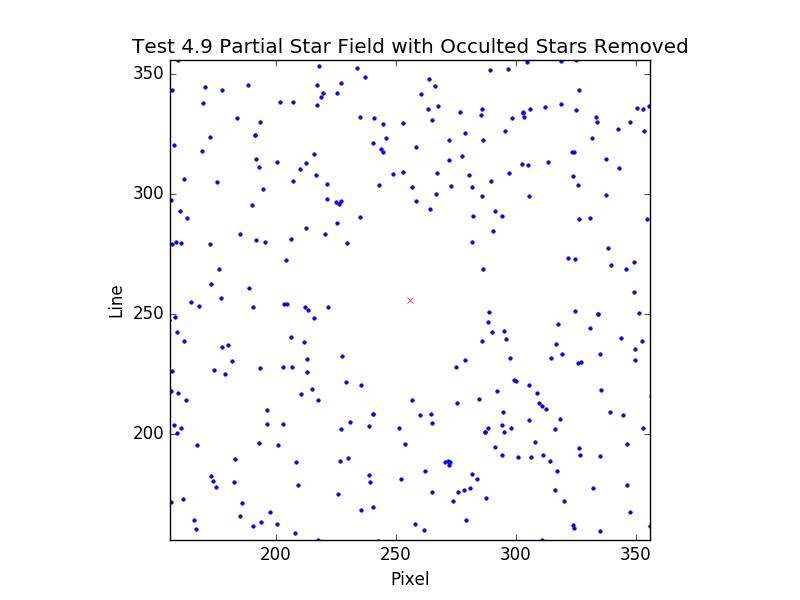
\includegraphics[height=2.25in]{partialWithHole}
    \end{subfigure}%
    ~ 
    \begin{subfigure}
        \centering
        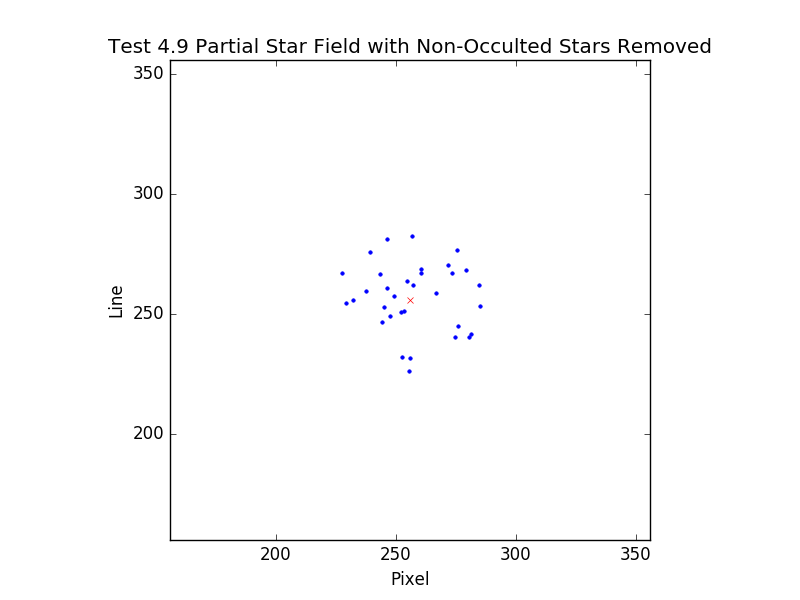
\includegraphics[height=2.25in]{partialWithFill}
    \end{subfigure}

    \caption{Zoomed images of test 4.9 star field. Images show set of non-occulted stars and set of occulted stars.}
    \label{512}
\end{figure*}
\begin{figure*}[t!]
    \centering
    \begin{subfigure}
        \centering
        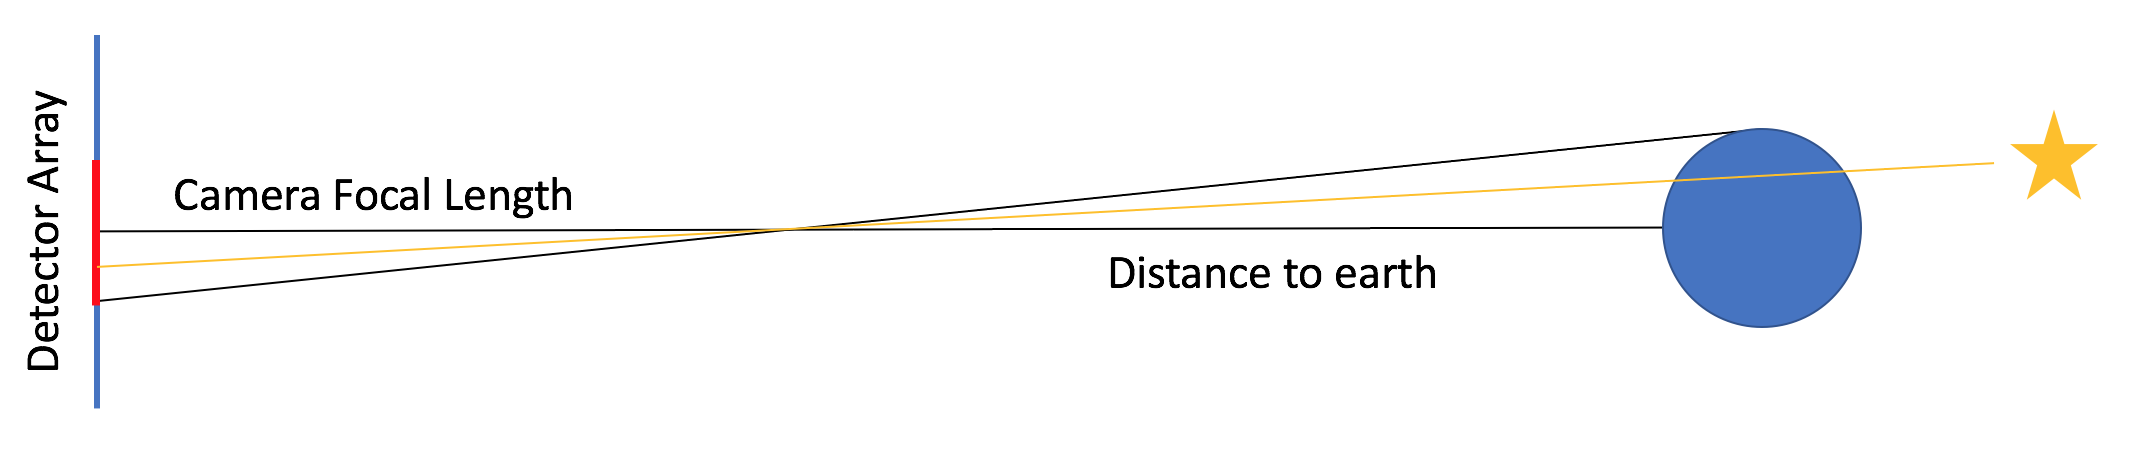
\includegraphics[width=6in]{occultedStar}
    \end{subfigure}%
    ~ 
    \begin{subfigure}
        \centering
        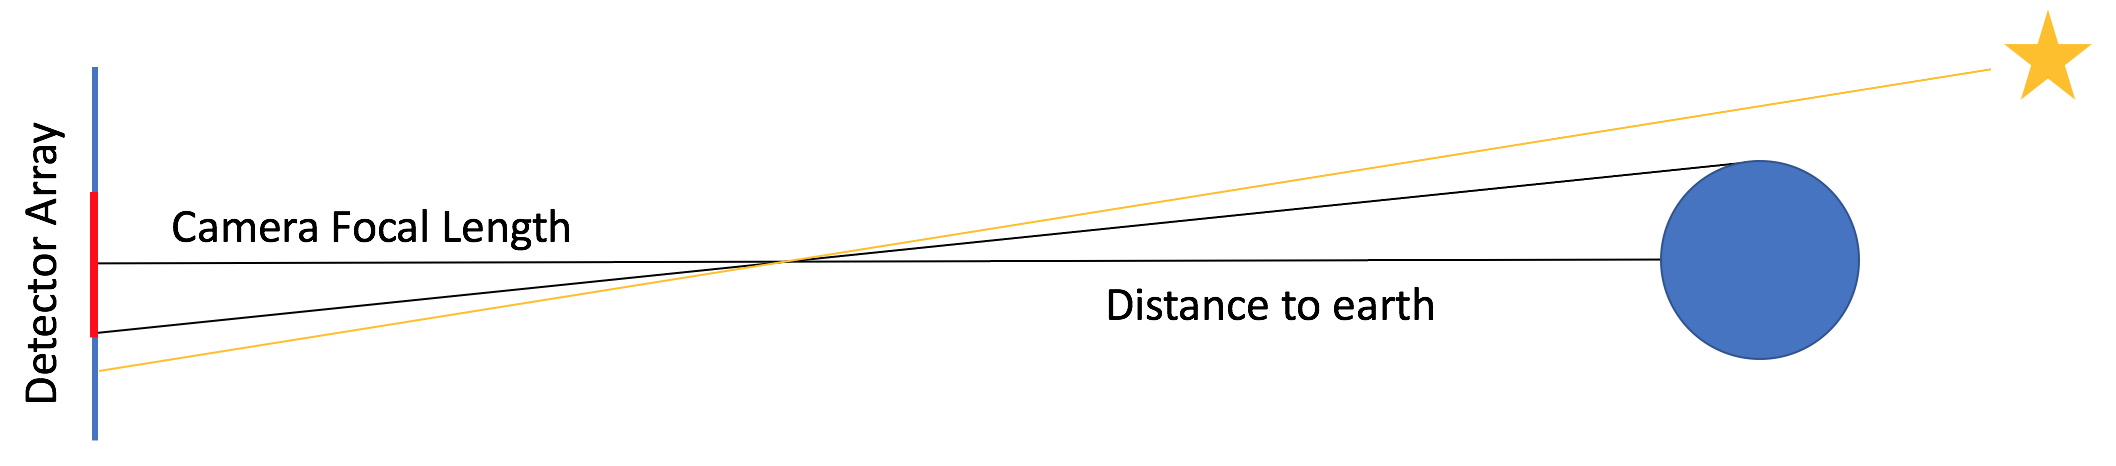
\includegraphics[width=6in]{nonOccultedStar}
    \end{subfigure}

    \caption{Cartoon showing the mapping of occulted and non-occulted stars onto the detector plane (blue). We see that the occuted star appears within the extended image of the Earth on the detector plane (red), and that the non-occulted star appears outside of the image of the Earth.}
    \label{512}
\end{figure*}

\subsection{Test 4.10: image.psf()}
\textbf{Status}: Incomplete. 10.31.17\\
\textbf{Responsible Team Member}: Matt Muszynski \\
\textbf{Description}: Because we expect the gaussian PDF applied to stars and body facets to be normalized, this test checks that the sum of the PSF caluclated by image.psf() is indeded one.\\
\textbf{Method}: \\

\subsection{Test 4.11: image.psf()}
\textbf{Status}: Incomplete. 10.31.17\\
\textbf{Responsible Team Member}: Matt Muszynski \\
\textbf{Description}: The PSF calculated at runtime should be centered at (0,0) in pixel/line space. This test ensures that it is.\\
\textbf{Method}: \\

\subsection{Test 4.12: image.psf()}
\textbf{Status}: Incomplete. 10.31.17\\
\textbf{Responsible Team Member}: Matt Muszynski \\
\textbf{Description}: This test fits a 2D gaussian to the PSF created my image.psf() at run time to enure the correct covariance is achieved.\\
\textbf{Method}: \\

\subsection{Test 4.13: image.rasterize()}
\textbf{Status}: Incomplete. 10.31.17\\
\textbf{Responsible Team Member}: Beryl Kuo \\
\textbf{Description}: \\
\textbf{Method}: \\

\subsection{Test 4.14: image.add\_read\_noise()}
\textbf{Status}: Incomplete. 10.31.17\\
\textbf{Responsible Team Member}: Ishaan Patel \\
\textbf{Description}: This test adds read noise to a blank image and ensures that it is in fact gaussian as desired.\\
\textbf{Method}: \\

\subsection{Test 4.15: image.add\_poisson\_noise()}
\textbf{Status}: Incomplete. 10.31.17\\
\textbf{Responsible Team Member}: Ishaan Patel \\
\textbf{Description}: This test adds poisson noise to a false detector array and checks the output to ensure it is truly a poisson distribution.\\
\textbf{Method}: \\

\subsection{Test 4.16: Image Pixel and Line Conversion}
\textbf{Status}: Incomplete. 10.31.17\\
\textbf{Responsible Team Member}: Matt Muszynski \\
\textbf{Description}: This method takes all stars from a scene, calculates their angular separation using their pixel and line coordinates and the physical characteristics of the camera that took the image. This is then compared to the true angular separation between the two stars using the dot product of the unit vector pointing at each.\\
\textbf{Method}: Test 4.16 leverages the same star field as test 4.9.
\begin{enumerate}
    \item Compute the distance between the center of the field of view and each star, both in the pixel direction and the line direction.
    \item Calculate the physical size of each pixel in pixel and line directions (physical size of the detector in that direction divided by the number of pixels in that direction)
    \item Compute the distance between the center of the field of view and each star on the detector plane in physical distance in pixel and line directions (multiply pixel distance by physical size in the pixel direction and line distance times the physical size of a pixel in the line direction).
    \item Calculate the true distance between the center of the FOV and each star in physical space (using Pythagorean theorem).
    \item Calculate the angular distance between the center of the FOV and each star by projecting using the physical distance between the two points and the focal length.
    \item Calculate the true angular distance between the center of the camera FOV and the star using dot products.
    \item Assert that both angualr distnaces are the same.
\end{enumerate}
\begin{figure*}[t!]
    \centering
    \begin{subfigure}
        \centering
        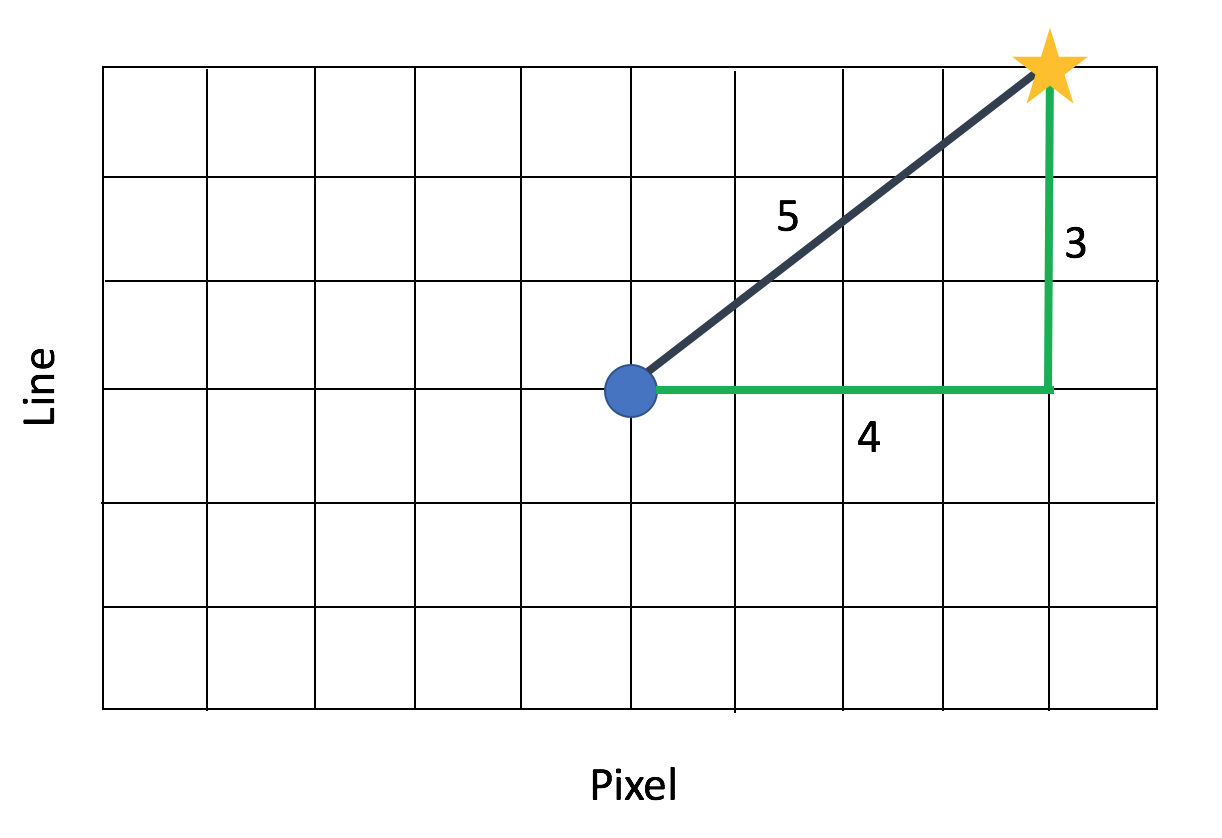
\includegraphics[width=2.5in]{detectorArr}
    \end{subfigure}%
    \caption{Here, the star appears 3 lines and 4 pixels away from the center of the FOV (blue dot). Assuming each pixel is 1 unit by 1 unit, this makes the star 5 units away from the center of the FOV. Test 4.16 shows that it does.}
    ~ 
    \begin{subfigure}
        \centering
        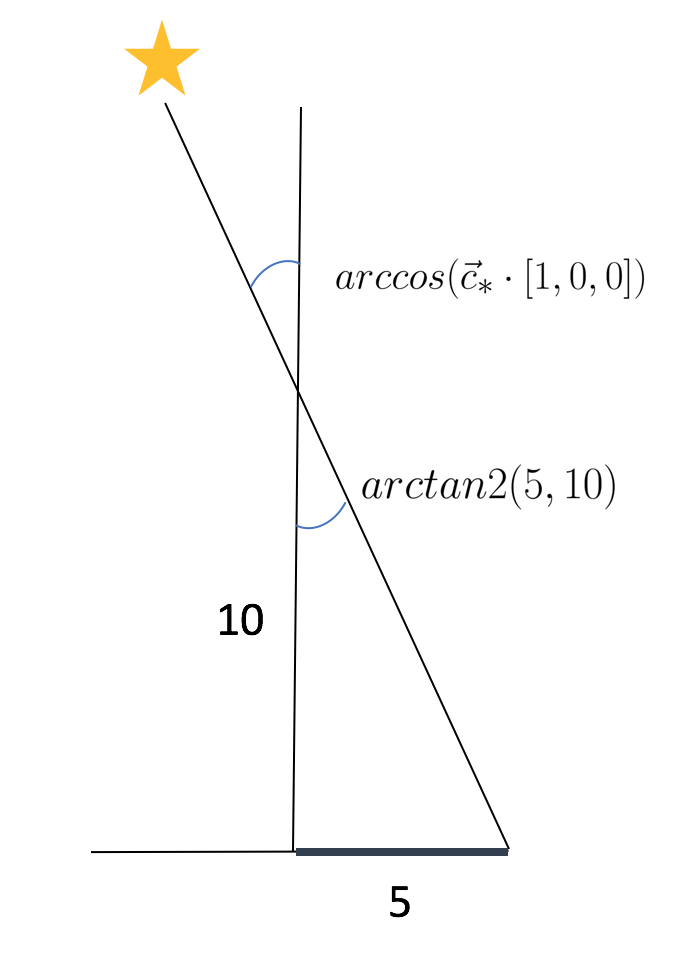
\includegraphics[width=2.5in]{projectedStar}
    \end{subfigure}
    \caption{Assuming that the focal length of the camera is 10 units, we can use arctan2 to find that the angular distance between the center of the FOV and the star must be 30 degrees. This must match the arccos of the dot product between the star's unit vector $\vec{c}_*$ and the boresite vector in camera coordinates, $[1,0,0]$}
\end{figure*}


\subsection{Test 4.17: em.planck()}
\textbf{Status}: Test Passes. 10.31.17\\
\textbf{Responsible Team Member}: Matt Muszynski \\
\textbf{Description}: This test checks that the value of the integral of em.planck() over all wavelength space to the output of em.stefan\_boltzmann() matches to within 0.1\% \\
\textbf{Method}: This method performs a numerical integration of the planck functon over a wavelength range of 1nm to 10000nm in 1nm bins. Values outside of this range are ignored as they are very small. This involves evaluating em.planck() at all wavelengths and multiplying by 1nm (essentially a Riemann sum). This then gives a value in units of $W/m^2/sr$. The $sr$ portion of this value can be removed by multiplying by a factor of pi (the solid angle subtended by the source as measured at the source). Theoretically this value should match the output of the stefan-boltzmann function exactly. In order to allow for the error inherent in the numerical integration, we only assert that the values match to within 0.1\%.\\

\subsection{Test 4.18: em.planck()}
\textbf{Status}: Test Passes. 10.31.17\\
\textbf{Responsible Team Member}: Matt Muszynski \\
\textbf{Pytest Function Name}: \\†
\textbf{Description}: This test checks that the value of the integral of em.planck() over all wavelength space to the accepted solar constant value of $1367 W/m^2$ to within 0.1\% \\
\textbf{Method}: The method for test 4.18 matches that of 4.17 through multiplying by the solid angle subtended by the source, which here does not reduce to pi, but is rather $\pi\frac{r^2_\astrosun}{a^2_\earth}$ where $a_\earth$ is the semi-major axis of Earth's orbit and $r_\astrosun$ is the radius of the sun. This gives the value of solar flux as measured from 1au, which is well characterized to be 1367 $W/m^2$. Again, we test that the computed value matches the accepted emprical value to within 0.1\%. \\
\end{document}
